% Authors: David Padilla Orenga, Ignacio Pastore Benaim
\documentclass{article}
\usepackage[utf8]{inputenc}
\usepackage[linesnumbered,ruled,vlined]{algorithm2e} 
\usepackage[a4paper, margin=1in, top=0.25in, bottom=1in, left=0.75in, right=0.75in]{geometry}
\title{Assignment 5 \\ \small Introduction to OpenCL programming.}
\author{David Padilla Orenga\\ Ignacio Pastore Benaim}
\date{}  

\usepackage{graphicx}
\usepackage{amsmath}
\usepackage{hyperref}
\usepackage{color}
\usepackage{subcaption}


% Hyphen penalty
\hyphenpenalty=10000
\exhyphenpenalty=10000
\sloppy

\begin{document}

\maketitle

\section*{Environment Setup}

The OpenCL environment was set up on a macOS system with the following specifications:

\begin{table}[h!]
\centering
\renewcommand{\arraystretch}{1.5} % Adjust row height
\begin{tabular}{|l|l|}
\hline
\textbf{Specification}                           & \textbf{Value}                         \\ \hline
Platform Name                                   & Apple                                  \\ \hline
Platform Vendor                                 & Apple                                  \\ \hline
Platform Version                                & OpenCL 1.2 (Feb 10 2024 00:43:19)     \\ \hline
Platform Host Timer Resolution                  & Not defined in OpenCL 1.2    \\ \hline
Number of Available Devices                     & 1                                      \\ \hline
Device Name                                     & Apple M1                               \\ \hline
Device Max Compute Units                        & 8                                      \\ \hline
Device Global Memory Cache Size                & 0 KB                                   \\ \hline
Device Global Memory Size                       & 5460 MB                                \\ \hline
Device Local Memory Size                        & 32 KB                                  \\ \hline
Device Max Work Group Size                      & 256                                    \\ \hline
Device Profiling Timer Resolution               & $1.0 \times 10^{3}$ nanoseconds        \\ \hline
\end{tabular}
\caption{OpenCL platform and device specifications}
\label{tab:platform_specs}
\end{table}

\section*{Sobel Edge Detection}

Sobel Edge Detection is a fundamental image processing algorithm that detects edges by computing intensity gradients
in horizontal and vertical directions. This assignment implements the algorithm in 
OpenCL to showcase the advantages of parallel processing.

\begin{figure}[h!]
\captionsetup[subfigure]{labelformat=empty}
    \centering
    \begin{minipage}{0.45\textwidth}
        \centering
        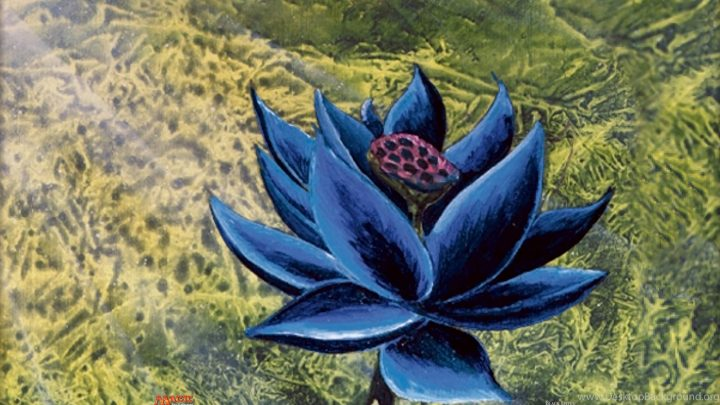
\includegraphics[width=\textwidth]{./images/input_blacklotus.jpg} % Replace with your input image
        \caption*{(a) Input Image}
    \end{minipage}
    \hfill
    \begin{minipage}{0.45\textwidth}
        \centering
        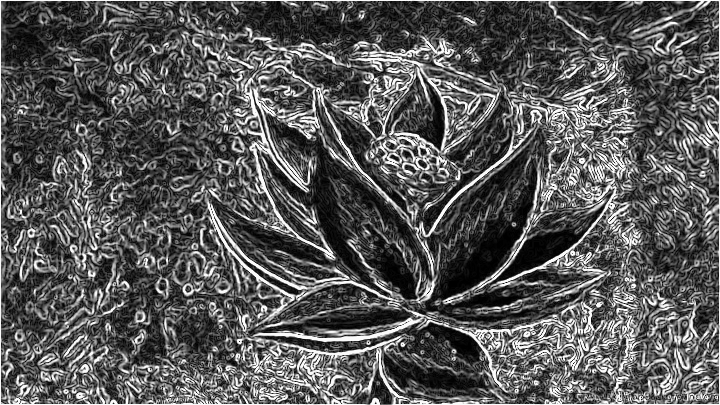
\includegraphics[width=\textwidth]{./images/output_blacklotus.jpg} % Replace with your output image
        \caption*{(b) Sobel Edge Detection Output}
    \end{minipage}
    \caption{Comparison of the input image and the result of Sobel Edge Detection.}
    \label{fig:sobel_comparison}
\end{figure}

\subsection*{Implementation Details}

The implementation involves two main components:
\begin{itemize}
    \item \textbf{Host Program:} The host program prepares input data, sets up the OpenCL environment, 
    and manages kernel execution. It also logs performance metrics and results.
    \item \textbf{Kernel Program:} The kernel performs convolution on image data, leveraging
     global and local memory for optimization. Shared memory was used to load blocks 
     of the image into faster memory for efficient access during computation.
\end{itemize}

The kernel was designed to process rectangular images, dynamically adjusting the 
global work size to match the image dimensions while ensuring compatibility with the local size. Halo regions 
were carefully handled to prevent edge artifacts during convolution.


\subsection*{Experiment Design}

The aim of this experiment was to implement Sobel Edge Detection and analyze its performance on both GPU and CPU platforms, with the CPU serving as a baseline for comparison. The following steps outline the experimental design:

\begin{itemize}
    \item \textbf{Input Images:} RGB images of various dimensions (\(256\times256\); \(256\times512\); \(512\times512\); 
    \(720\times1280\); \(1024\times1024\); and \(2048\times4096\)) were generated using the CImg library. These images were converted to grayscale as input for the Sobel filter.
    \item \textbf{CPU Implementation:} The CPU implementation calculates the Sobel gradients sequentially, 
    measuring both the total execution time and computation-only time for each run.
    \item \textbf{GPU Implementation:} The GPU implementation leverages OpenCL to parallelize the Sobel filter. 
    Tests were conducted using different local sizes (\(2 \times 2\); \(4 \times 4\); \(8\times 8\) and \(16 \times 16\) ), 
    chosen based on the device’s local memory size of \(32\,\mathrm{KB}\), to optimize performance.
\end{itemize}

The choice of these dimensions ensures coverage of a variety of image sizes, simulating small and large-scale input data. Testing with increasing local sizes enables evaluation of GPU memory usage and processing efficiency. Input images were created with the CImg library as shown in Figure \ref{fig:input_output_comparison}.

\begin{figure}[h!]
    \captionsetup[subfigure]{labelformat=empty}
        \centering
        \begin{minipage}{0.45\textwidth}
            \centering
            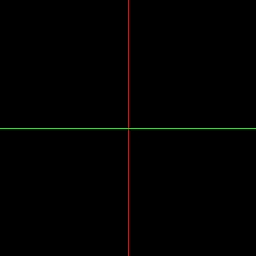
\includegraphics[width=\textwidth]{./images/input_256x256.jpg} % Replace with your input image
            \caption*{(a) Input for profiling (256x256)}
        \end{minipage}
        \hfill
        \begin{minipage}{0.45\textwidth}
            \centering
            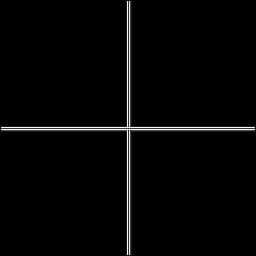
\includegraphics[width=\textwidth]{./images/output_256x256.jpg} % Replace with your output image
            \caption*{(b) Sobel output for profiling (256x256)}
        \end{minipage}
        \caption{Example input and output images for Sobel Edge Detection.}
        \label{fig:input_output_comparison}
    \end{figure}

\subsection*{CPU Execution Times}

CPU execution times were measured for each input image. 
Both the total execution time, including data preparation, and 
the computation-only time for applying the Sobel filter were logged.

\subsection*{GPU Measures}

The GPU implementation was evaluated for each image size across multiple local sizes. 

Metrics recorded include:

\begin{itemize}
    \item \textbf{Total Execution Time:} Time from data preparation to result output. This is the overall time measured for the entire process, including any overhead.

    \item \textbf{Kernel Execution Time:} Time taken for the kernel to process the input image. This excludes the data transfer time and focuses solely on the computation.

    \item \textbf{Throughput:} The number of pixels processed per second, calculated using the formula:
    \[
    \text{Throughput} = \frac{\text{Width} \times \text{Height}}{\text{Kernel Execution Time (s)}}
    \]
    Where:
    \begin{itemize}
        \item \(\text{Width} \times \text{Height}\) is the total number of pixels in the image.
        \item \(\text{Kernel Execution Time (s)}\) is the time taken by the kernel in seconds, obtained by converting milliseconds to seconds as \(\text{Kernel Execution Time (ms)} \times 10^{-3}\).
    \end{itemize}

    \item \textbf{Memory Bandwidth:} The amount of data transferred per second during kernel execution, calculated as:
    \[
    \text{Bandwidth} = \frac{\text{Width} \times \text{Height} \times \text{sizeof(float)}}{\text{Kernel Execution Time (s)}}
    \]
    Where:
    \begin{itemize}
        \item \(\text{Width} \times \text{Height}\) is the total number of pixels.
        \item \(\text{sizeof(float)}\) represents the size of each pixel in bytes.
        \item \(\text{Kernel Execution Time (s)}\) is the execution time in seconds.
    \end{itemize}


\end{itemize}

\section*{Results and Analysis}

\subsection*{GPU Execution Times}
The figures \ref{fig:kernel_exec} and \ref{fig:program_exec} show the kernel and 
program execution times for different local sizes and image dimensions.

\begin{figure}[h!]
    \centering
    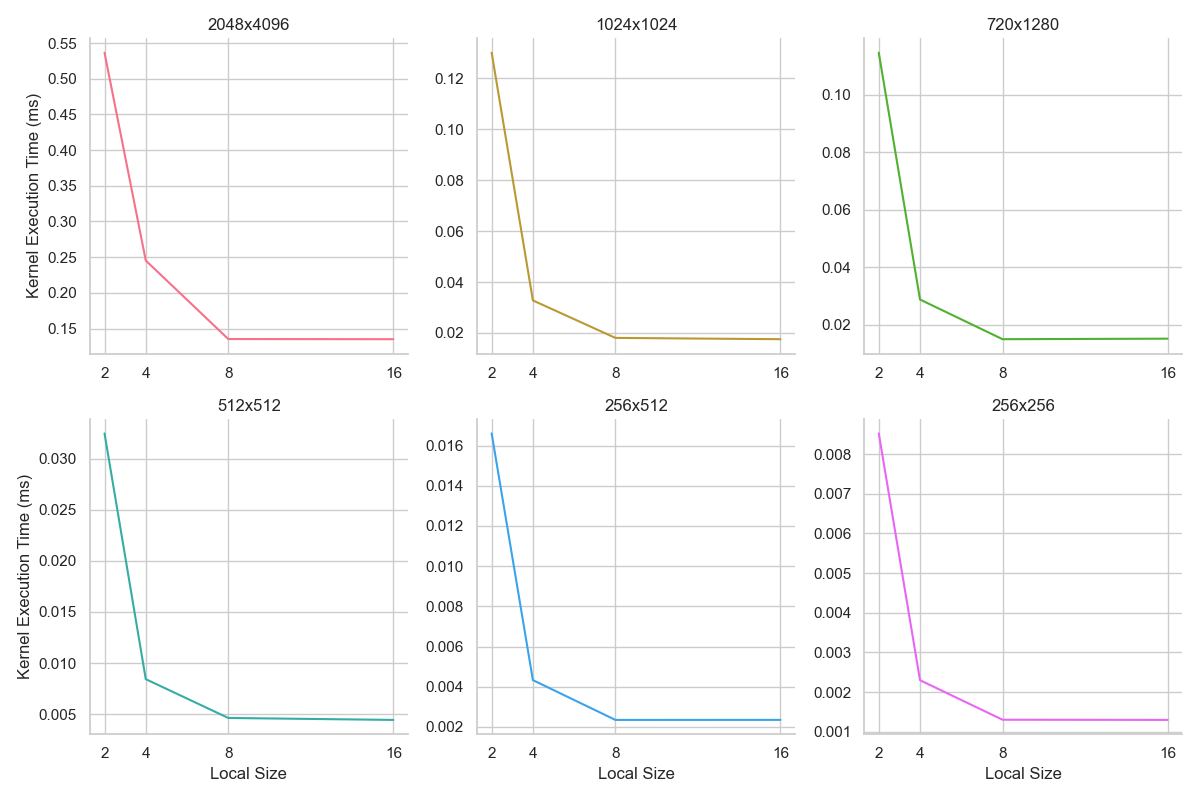
\includegraphics[width=\textwidth]{./images/kernel_exec.png}
    \caption{Kernel Execution Time vs Local Size for various image dimensions.}
    \label{fig:kernel_exec}
\end{figure}

\begin{figure}[h!]
    \centering
    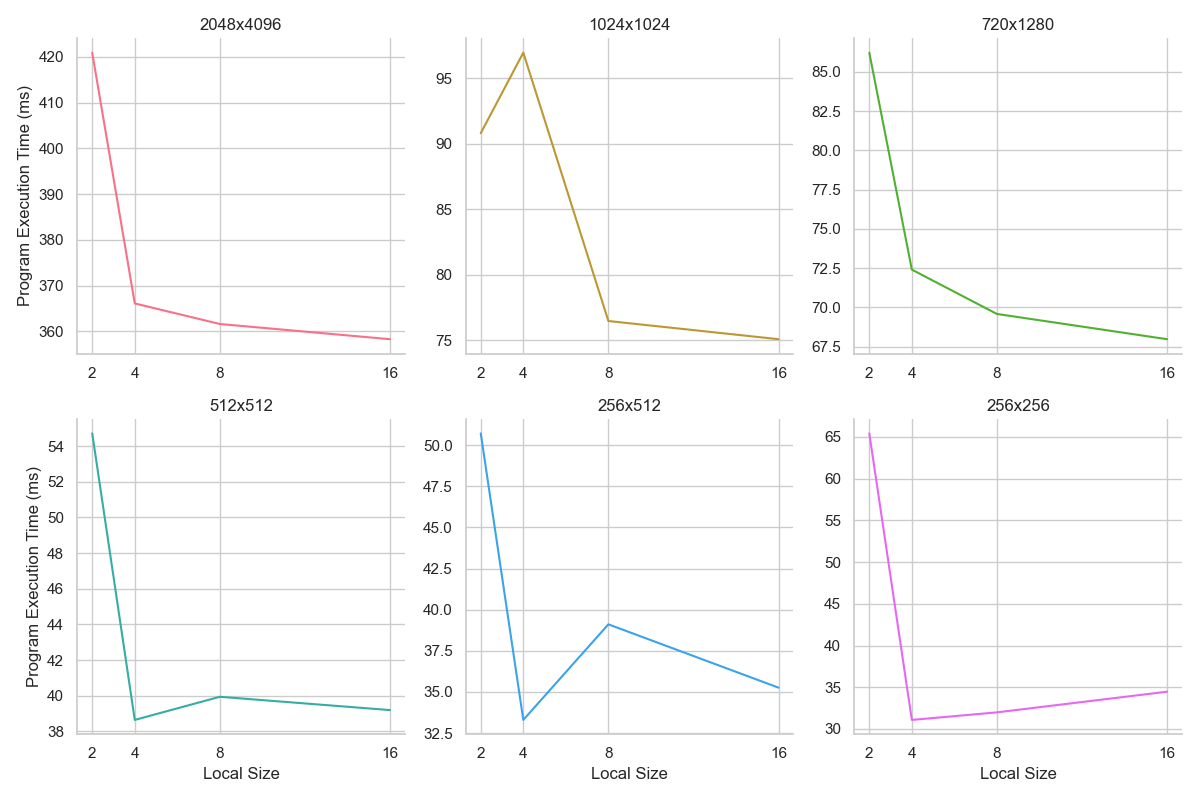
\includegraphics[width=\textwidth]{./images/program_exec.png}
    \caption{Program Execution Time vs Local Size for various image dimensions.}
    \label{fig:program_exec}
\end{figure}

%% Add an analysis here
In all cases the kernel execution times decreases as the local size increases. Also, there is a clear tendency for the program execution time to decrease as the local size increases. This is expected because larger local sizes reduce the overhead of managing smaller workgroups and improve resource utilization on the GPU.

Certain configurations, such as the \(1024 \times 1024\) image at a local size of \(4 \times 4\) and the \(256 \times 512\)image at a local size of \(4\times 4\), show notable peaks in execution time. These peaks likely represent overhead introduced by suboptimal partitioning of the workload or inefficient use of GPU resources at these specific local sizes.

\subsection*{CPU Execution Times}
The total execution time and kernel execution time for CPU implementation are presented in Figure~\ref{fig:cpu_exec}.

\begin{figure}[h!]
    \centering
    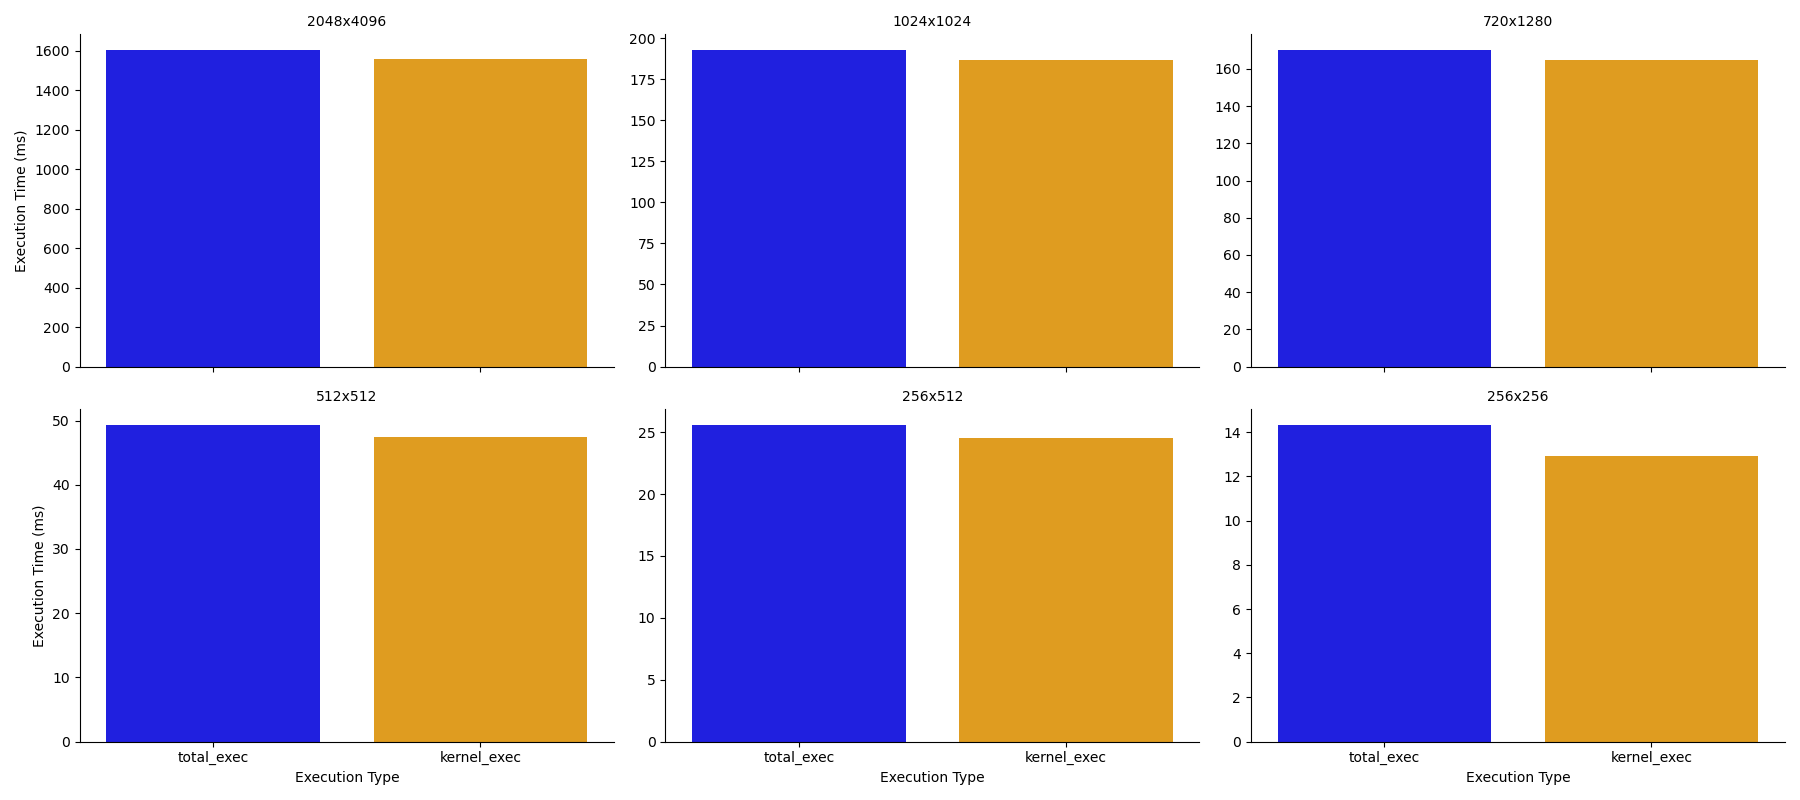
\includegraphics[width=\textwidth]{./images/cpu_exec.png}
    \caption{Comparison of Total and Kernel Execution Times for CPU.}
    \label{fig:cpu_exec}
\end{figure}

First, we can see that the kernel execution time is the dominant factor in the total execution time, indicating that the computation is the bottleneck in the CPU implementation. Moreover, in comparison with the GPU implementation, the CPU execution
times are significantly higher than the optimal GPU execution times for large scle images, highlighting the superior performance of the GPU for parallel processing tasks. We can also observe that for small images like \(256 \times 256\) or \(256 \times 512\), the CPU execution times are comparable to the GPU execution times, suggesting that the CPU is more efficient for smaller datasets.

\subsection*{Performance Analysis}
Since the selected metrics only vary with the kernel execution time, we decided to display only
the performance metrics for the \(16 \times 16\) local size. Table~\ref{tab:performance_metrics} summarizes the performance metrics for various image dimensions.

\begin{table}[h!]
\centering
\renewcommand{\arraystretch}{1.3}
\begin{tabular}{|c|c|c|c|}
\hline
\textbf{Image Dimension} & \textbf{Bandwidth (GB/s)} & \textbf{Throughput (\( \times 10^9\) pixels/s)}  \\ \hline
2048x4096                & 248.49                     & 62.12                                            \\ \hline
1024x1024                & 239.48                     & 59.87                                            \\ \hline
720x1280                 & 242.45                     & 60.61                                            \\ \hline
512x512                  & 236.67                     & 59.17                                            \\ \hline
256x512                  & 223.29                     & 55.82                                            \\ \hline
256x256                  & 202.06                     & 50.52                                            \\ \hline

\end{tabular}
\caption{Performance metrics for various image dimensions. Bandwidth is converted to GB/s, throughput is expressed in billions of pixels per second.}
\label{tab:performance_metrics}
\end{table}

From the table, it is evident that larger images, such as \(2048 \times 4096\), exhibit higher throughput and bandwidth, highlighting the GPU's capability to efficiently handle large datasets. This demonstrates the scalability of the GPU for parallel processing tasks as the dataset size increases. In contrast, smaller images, such as \(256 \times 256\), have significantly lower memory requirements but still maintain notable throughput levels. However, the bandwidth utilization is comparatively reduced for these smaller datasets, indicating that the GPU is not fully utilized under such conditions. This suggests that the GPU performs optimally with larger workloads, where its parallel processing capabilities can be fully leveraged.


\end{document}